\chapter{Modules} \label{chap:modules}
% Structure of base module description
% - definovat nezavislost 
% - define config files (JSON, structure)
% - define communication by WebSocket and MQTT (topics)

% Structure of each module:
% - description
% - commands and responses
% - communicating with who
% - next used technology (fritzing, mongoDB, etc.)

Modules are well-encapsulated code written to provide functional and control elements (moves) above home to the user. Each module inherits from VoicehomeModule class that provide communicating interface to each module by WebSocket, MQTT and mediate writing and reading from MongoDB. Each module defines its topic for MQTT and a passport for WebSocket that subscribe from these services. Messages containing these topics or passports are passed through the engine to the modules.

Thus each module has to be created by the following approach:

\begin{enumerate}[label=\arabic*)]
    \item Create a new folder in \texttt{"voicehome\textbackslash modules\textbackslash "}, the name of this folder is the module's name.
    \item Create two mandatory files
    \begin{enumerate}
        \item \texttt{"voicehome\textbackslash modules\textbackslash <module\_name>\textbackslash metadata.json"} that include object with following variables.
        \begin{itemize}
            \item \texttt{"module\_id"}: contain the name of the module
            \item \texttt{"description"}: contain a string with a brief description of the module
            \item \texttt{"mqtt\_topics"}: contain a list of MQTT topics module wants to subscribe
            \item \texttt{"websocket\_passports"}: contain a list of WebSocket passports passing messages to the module
            \item \texttt{"moves"}: list of objects that define moves this module is capable of
            \begin{itemize}
                \item \texttt{"move\_id"}: a unique ID that follows the convention \texttt{<module\_name>\_<order\_in\_this\_list>}
                \item \texttt{"method\_name"}: contain the name of a Python function in \texttt{<module\_name>.py} called when this move is activated
                \item \texttt{"description"}: contain a brief description of the move
                \item \texttt{"calls"}: list of calls (voice commands to VoiceKit) activating this move; it is a list of lists of words (must fit the chosen logic algorithm)
            \end{itemize}
        \end{itemize}
        \item \texttt{"voicehome/modules/<module\_name>/<module\_name>.py"} that define class of module. This class have to inherit from VoicehomeModule and include all methods listed in the previous file \texttt{metadata.json}.
        
        \lstinputlisting[language=python,firstnumber=1,caption={Template for creating a new module},captionpos=b, label={lst:regex_python}]{code/module_class_template.py}
    \end{enumerate}
\end{enumerate}

After accomplishing these requirements, it is not necessary to restart the entire engine but can simply use the voice command \texttt{"načti moduly"} from the System module. Each particular module can be turned off or on using the web interface in the Modules tab, which is specified in more detail in Chap. ***.

\section{Lights}

The system module provides the user commands to control lights by voice. The user not only turns on, off or blinks lights but can also identify the development boards by lighting a onboard LED on a specific board. The module keeps in memory a list of all lights with their current status and detailed description.

The onboard LEDs are mounted on the board from the factory on pin 2. The other lights have their specific wiring, but one LED is prepared for demonstration purposes, which by our definition is located in the living room and is wired according to the diagram in \cref{fig:led_schema}. 

\begin{figure}[H]
	\centering
	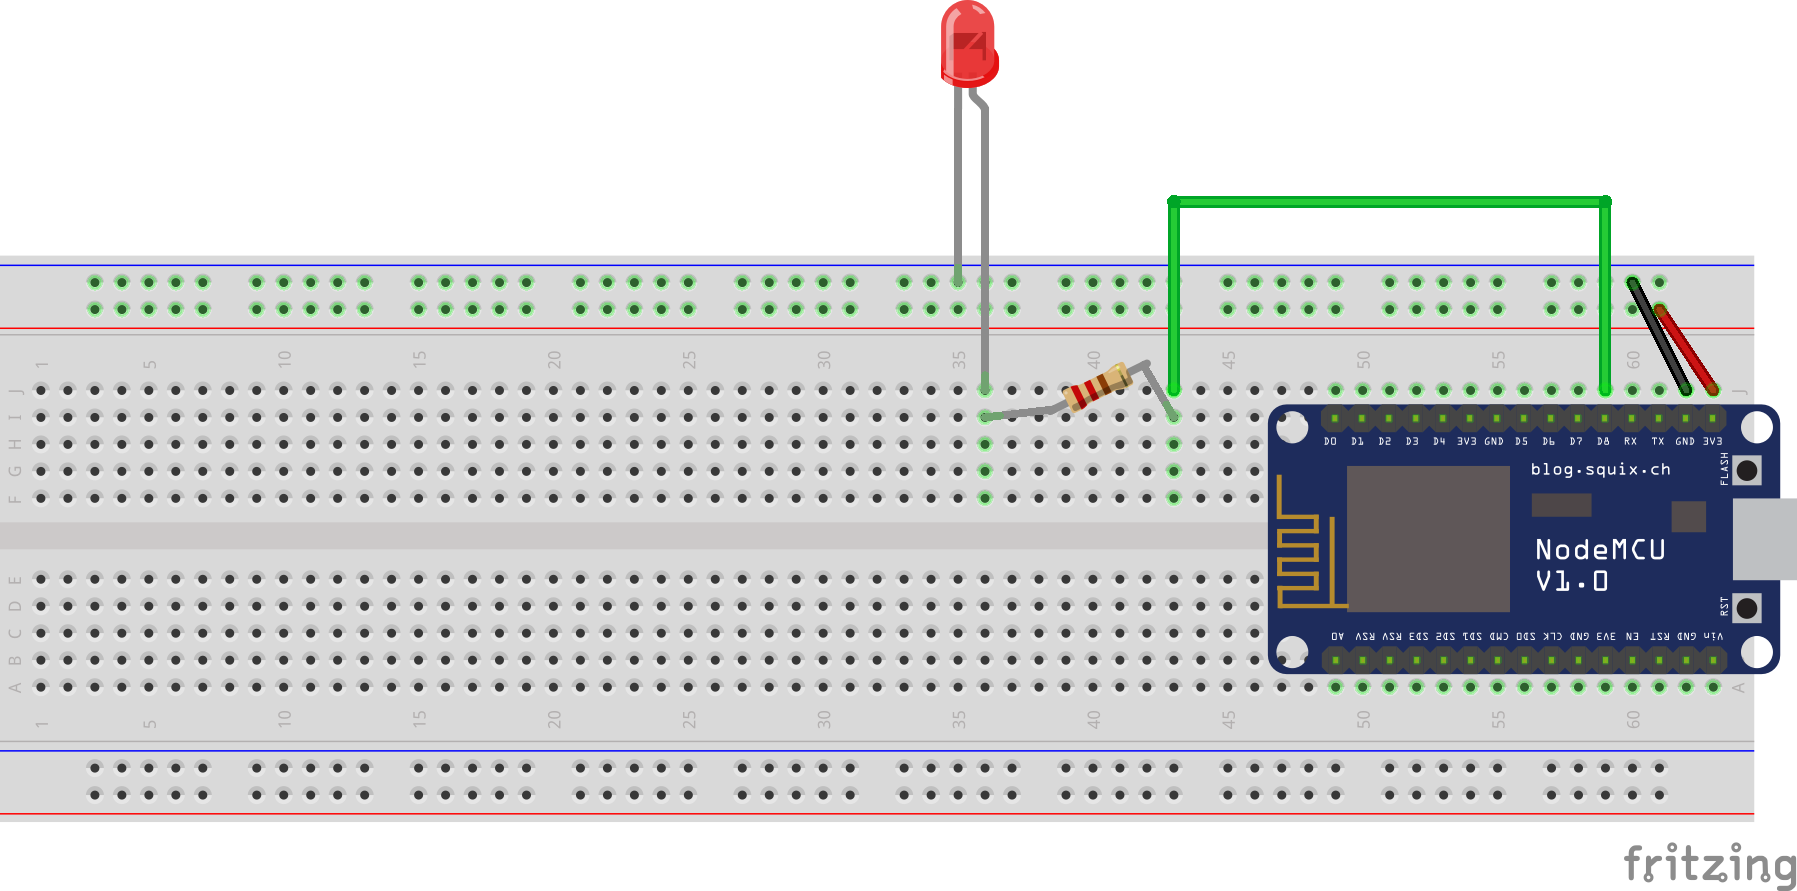
\includegraphics[width=\textwidth]{img/led_schema.png}
	\caption{LED "living room" wiring diagram}
	\label{fig:led_schema}
\end{figure}

% Uvidíš ke konci psaní, jak ti vycházejí stránky atd., ale možná bych zapřemýšlel nad tím, dát tyto kompletní seznamy voice commands také do appendixu a sem do hlavního textu dát např. jen tabulku s anglickými názvy moves, případně s anglickým description of move a přidat odkaz na tento kompletní seznam.

\subsection{Voice commands}
The module responds to the following questions:
\begin{itemize}
    \item Turn on all the onboard LEDs\\
    \textbf{Voice commands}
    \begin{itemize}
        \item "Rozsviť všechny vývojové desky."
        \item "Rozsviť všechny vestavěné ledky."
    \end{itemize}
    \textbf{Reply}
    \begin{itemize}
        \item Module confirm each light separately - "Vývojová deska jedna je rozsvícena.", "Vývojová deska dva je rozsvícena.", etc.
    \end{itemize}
    \item Turn off all the onboard LEDs\\
    \textbf{Voice commands}
    \begin{itemize}
        \item "Zhasni všechny vývojové desky."
        \item "Zhasni všechny vestavěné ledky."
    \end{itemize}
    \textbf{Reply}
    \begin{itemize}
        \item Module confirm each light separately - "Vývojová deska jedna je zhasnuta.", "Vývojová deska dva je zhasnuta.", etc.
    \end{itemize}    
    \item Turn on the light 1\\
    \textbf{Voice commands}
    \begin{itemize}
        \item "Zapni obýváku světlo."
        \item "Rozsviť obýváku světlo."
        \item "Zapni obývacím pokoji světlo."
        \item "Rozsviť obývacím pokoji světlo."
    \end{itemize}
    \textbf{Reply}
    \begin{itemize}
        \item "Světlo v obývacím pokoji rozsvíceno."
    \end{itemize} 
    \item Turn off the light 1\\
    \textbf{Voice commands}
    \begin{itemize}
        \item "Vypni obýváku světlo."
        \item "Zhasni obýváku světlo."
        \item "Vypni obývacím pokoji světlo."
        \item "Zhasni obývacím pokoji světlo."
    \end{itemize}
    \textbf{Reply}
    \begin{itemize}
        \item "Světlo v obývacím pokoji zhasnuto."
    \end{itemize} 
    \item Turn on the onboard LED number 1\\
    \textbf{Voice commands}
    \begin{itemize}
        \item "Rozsviť vestavěnou ledku vývojové desky číslo jedna."
        \item "Rozsviť vývojovou desku číslo jedna."
    \end{itemize}
    \textbf{Reply}
    \begin{itemize}
        \item "Vývojová deska číslo jedna rozsvícena."
    \end{itemize} 
    \item Turn off the onboard LED number 1\\
    \textbf{Voice commands}
    \begin{itemize}
        \item "Zhasni vestavěnou ledku vývojové desky číslo jedna."
        \item "Zhasni vývojovou desku číslo jedna."
    \end{itemize}
    \textbf{Reply}
    \begin{itemize}
        \item "Vývojová deska číslo jedna zhasnuta."
    \end{itemize}
    \item Turn on the onboard LED number 2\\
    \textbf{Voice commands}
    \begin{itemize}
        \item "Rozsviť vestavěnou ledku vývojové desky číslo dva."
        \item "Rozsviť vývojovou desku číslo dva."
    \end{itemize}
    \textbf{Reply}
    \begin{itemize}
        \item "Vývojová deska číslo dva rozsvícena."
    \end{itemize}
    \item Turn off the onboard LED number 2\\
    \textbf{Voice commands}
    \begin{itemize}
        \item "Zhasni vestavěnou ledku vývojové desky číslo dva."
        \item "Zhasni vývojovou desku číslo dva."
    \end{itemize}
    \textbf{Reply}
    \begin{itemize}
        \item "Vývojová deska číslo dva zhasnuta."
    \end{itemize}
    \item Turn on the onboard LED number 3\\
    \textbf{Voice commands}
    \begin{itemize}
        \item "Rozsviť vestavěnou ledku vývojové desky číslo tři."
        \item "Rozsviť vývojovou desku číslo tři."
    \end{itemize}
    \textbf{Reply}
    \begin{itemize}
        \item "Vývojová deska číslo tři rozsvícena."
    \end{itemize}
    \item Turn off the onboard LED number 3\\
    \textbf{Voice commands}
    \begin{itemize}
        \item "Zhasni vestavěnou ledku vývojové desky číslo tři."
        \item "Zhasni vývojovou desku číslo tři."
    \end{itemize}
    \textbf{Reply}
    \begin{itemize}
        \item "Vývojová deska číslo tři zhasnuta."
    \end{itemize}
    \item Voicekit answer which lights are turned on\\
    \textbf{Voice commands}
    \begin{itemize}
        \item "Která světla svítí."
    \end{itemize}
    \textbf{Reply}
    \begin{itemize}
        \item "Aktuálně nejsou rozsvícena žádná světla."
        \item "Aktuálně jsou rozsvícena tyto světla první ESP, druhé ESP..."
    \end{itemize}
\end{itemize}

\subsection{Messages structure}
The engine uses for maintain lights following topics and messages:

\begin{itemize}
    \item "voicehome/lights/command" - to turn the light on/off
    \begin{lstlisting}[language=json,firstnumber=1,caption={Structure of JSON message to turn on/off the light in module \textit{Lights}},captionpos=b,xleftmargin=1cm]
{
    "ID":1,
    "type":"ESP_onboard",
    "set":0
}
    \end{lstlisting}
    \item "voicehome/lights/state/command" - to ask the light for state
    \begin{lstlisting}[language=json,firstnumber=1,caption={Structure of JSON message to asking for the state of the light in module \textit{Lights}},captionpos=b,xleftmargin=1cm]
{
    "ID":1,
    "type":"ESP_onboard"
}
    \end{lstlisting}
    \item "voicehome/lights/state/receive" - to receive state of the light
    \begin{lstlisting}[language=json,firstnumber=1,caption={Structure of JSON message to receive state of the light in module \textit{Lights}},captionpos=b,xleftmargin=1cm]
{
    "type":"light",
    "state":0,
    "ID":1
}
    \end{lstlisting}
\end{itemize}

\section{Sensors}

The sensors module provides the user commands to communicate directly with sensors wired to the ESP development board or ask for statistics information such as average. The sensors connected to the module are bme280 (see \cref{fig:bme280_schema}), ds18b20 (see \cref{fig:ds18b20_schema}) and tsl2591 (see \cref{fig:tsl2591_schema}). The module uses the Python library to obtain old data from the MongoDB database to calculate statistical data.

\begin{itemize}
    \item Sends a command via MQTT to measure current temperature\\
    \textbf{Voice commands}
    \begin{itemize}
        \item "Kolik je stupňů?"
        \item "Jaká je teplota?"
        \item "Změř teplotu."
    \end{itemize}
    \textbf{Reply}
    \begin{itemize}
        \item "Na senzor je odeslán dotaz. Aktuální teplota je dvacet."
    \end{itemize}
    \item Sends a command via MQTT to measure current pressure\\
    \textbf{Voice commands}
    \begin{itemize}
        \item "Kolik je tlak?"
        \item "Jaký je tlak?"
        \item "Změř tlak."
    \end{itemize}
    \textbf{Reply}
    \begin{itemize}
        \item "Na senzor je odeslán dotaz. Aktuální tlak je devět set devadesát devět."
    \end{itemize}
    \item Sends a command via MQTT to measure current humidity\\
    \textbf{Voice commands}
    \begin{itemize}
        \item "Kolik je vlhkost?"
        \item "Jaká je vlhkost?"
        \item "Změř vlhkost."
    \end{itemize}
    \textbf{Reply}
    \begin{itemize}
        \item "Na senzor je odeslán dotaz. Aktuální vlhkost je deset."
    \end{itemize}
    \item Sends a command via MQTT to measure current illuminance\\
    \textbf{Voice commands}
    \begin{itemize}
        \item "Kolik je intenzity světla?"
        \item "Jaká je intenzita světla?"
        \item "Změř světlo."
    \end{itemize}
    \textbf{Reply}
    \begin{itemize}
        \item "Na senzor je odeslán dotaz. Aktuální intenzita světla je třicet."
    \end{itemize}
    \item Voicekit answer average temperature for the last day\\
    \textbf{Voice commands}
    \begin{itemize}
        \item "Průměrná teplota za poslední den."
        \item "Dnešní průměrná teplota."
    \end{itemize}
    \textbf{Reply}
    \begin{itemize}
        \item "Teplotu nebylo možné vypočíst."
        \item "Průměrná teplota za poslední den je dvacet."
    \end{itemize}
    \item Voicekit answer average pressure for the last day\\
    \textbf{Voice commands}
    \begin{itemize}
        \item "Průměrný tlak za poslední den."
        \item "Dnešní průměrný tlak."
    \end{itemize}
    \textbf{Reply}
    \begin{itemize}
        \item "Tlak nebylo možné vypočíst."
        \item "Průměrný tlak za poslední den je devět set devadesát."
    \end{itemize}
    \item Voicekit answer average humidity for the last day\\
    \textbf{Voice commands}
    \begin{itemize}
        \item "Průměrná vlhkost za poslední den."
        \item "Dnešní průměrná vlhkost."
    \end{itemize}
    \textbf{Reply}
    \begin{itemize}
        \item "Vlhkost nebylo možné vypočíst."
        \item "Průměrná vlhkost za poslední den je devět set devadesát."
    \end{itemize}
    \item Voicekit answer average illuminance for the last day\\
    \textbf{Voice commands}
    \begin{itemize}
        \item "Průměrná intenzita světelnosti za poslední den."
        \item "Dnešní průměrná intenzita světelnosti."
    \end{itemize}
    \textbf{Reply}
    \begin{itemize}
        \item "Světelnost nebylo možné vypočíst."
        \item "Průměrná intenzita světelnosti za poslední den je dvanáct."
    \end{itemize}
    \item Voicekit answer average temperature for the last week\\
    \textbf{Voice commands}
    \begin{itemize}
        \item "Průměrná teplota za poslední týden."
        \item "Týdenní průměrná teplota."
    \end{itemize}
    \textbf{Reply}
    \begin{itemize}
        \item "Teplotu nebylo možné vypočíst."
        \item "Průměrná teplota za poslední týden je dvacet."
    \end{itemize}
    \item Voicekit answer average pressure for the last week\\
    \textbf{Voice commands}
    \begin{itemize}
        \item "Průměrný tlak za poslední týden."
        \item "Týdenní průměrný tlak."
    \end{itemize}
    \textbf{Reply}
    \begin{itemize}
        \item "Tlak nebylo možné vypočíst."
        \item "Průměrný tlak za poslední týden je devět set devadesát."
    \end{itemize}
    \item Voicekit answer average humidity for the last week\\
    \textbf{Voice commands}
    \begin{itemize}
        \item "Průměrná vlhkost za poslední týden."
        \item "Týdenní průměrná vlhkost."
    \end{itemize}
    \textbf{Reply}
    \begin{itemize}
        \item "Vlhkost nebylo možné vypočíst."
        \item "Průměrná vlhkost za poslední týden je devět set devadesát."
    \end{itemize}
    \item Voicekit answer average illuminance for the last week\\
    \textbf{Voice commands}
    \begin{itemize}
        \item "Průměrná intenzita světelnosti za poslední týden."
        \item "Týdenní průměrná intenzita světelnosti."
    \end{itemize}
    \textbf{Reply}
    \begin{itemize}
        \item "Světelnost nebylo možné vypočíst."
        \item "Průměrná intenzita světelnosti za poslední týden je dvanáct."
    \end{itemize}
\end{itemize}

\subsection{BME280}

The BME280 \citep{BME280:Datasheet} module is used to measure the internal temperature and barometric pressure. In addition, our variant has a humidity sensor, which could not be put into operation, probably due to a defective piece. The measuring range of this sensor is in case of ambient temperature from -40 $^{\circ}$C to +85 $^{\circ}$C, in case of humidity from 0$\%$ to 100$\%$ and in case of barometric pressure from 300 hPa to 1100 hPa. Temperature values are measured with an accuracy of ± 1 $^{\circ}$C, humidity values with an accuracy of ± 3$\%$ and barometric pressure values with an accuracy of ± 1 Pa. The sensor is supplied with power from a 3.3 V output on the microchip and grounded to the microchip. The SDA and SCL outputs are wired to the D6 and D5 pins of the microchip to provide I2C communication. The wiring diagram of the TSL2591 sensor is shown in \cref{fig:bme280_schema}

\begin{figure}[H]
	\centering
	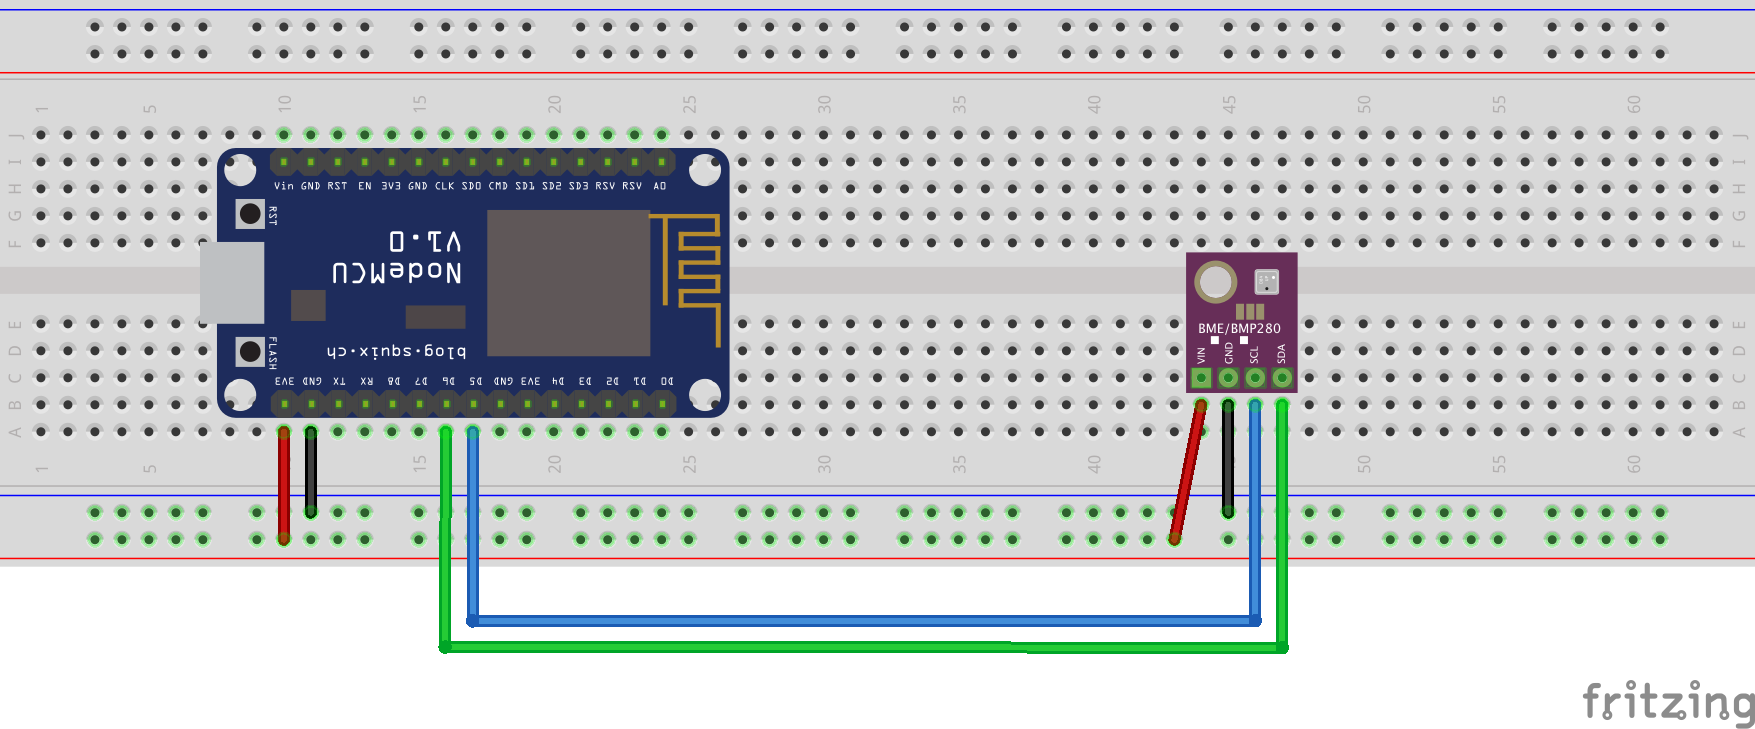
\includegraphics[width=\textwidth]{img/bme280_schema.png}
	\caption{BME 280 wiring diagram}
	\label{fig:bme280_schema}
\end{figure}


\subsection{DS18B20}

The DS18B20 \citep{DS18B20:Datasheet} is a temperature sensor, and its waterproof variant was chosen as an illustration.  The module's output is the value of temperature in the degree Celsius unit. The sensor's measuring range is from -55 to +125 degrees with an accuracy of ± 0,5 $^{\circ}$C within limits from -10 $^{\circ}$C to +85 $^{\circ}$C. The sensor communicates via the One-Wire interface and uses one pin for data transmission. The sensor is connected to the microchip by three wires - one wire for power supply 3,3V, one for grounding and one for data communication. It is necessary to connect a resistor of resistance 4.7 k$\Omega$ to the circuit, connecting the data and power wires. The wiring diagram of the DS18B20 sensor is shown in \cref{fig:ds18b20_schema}

\begin{figure}[H]
	\centering
	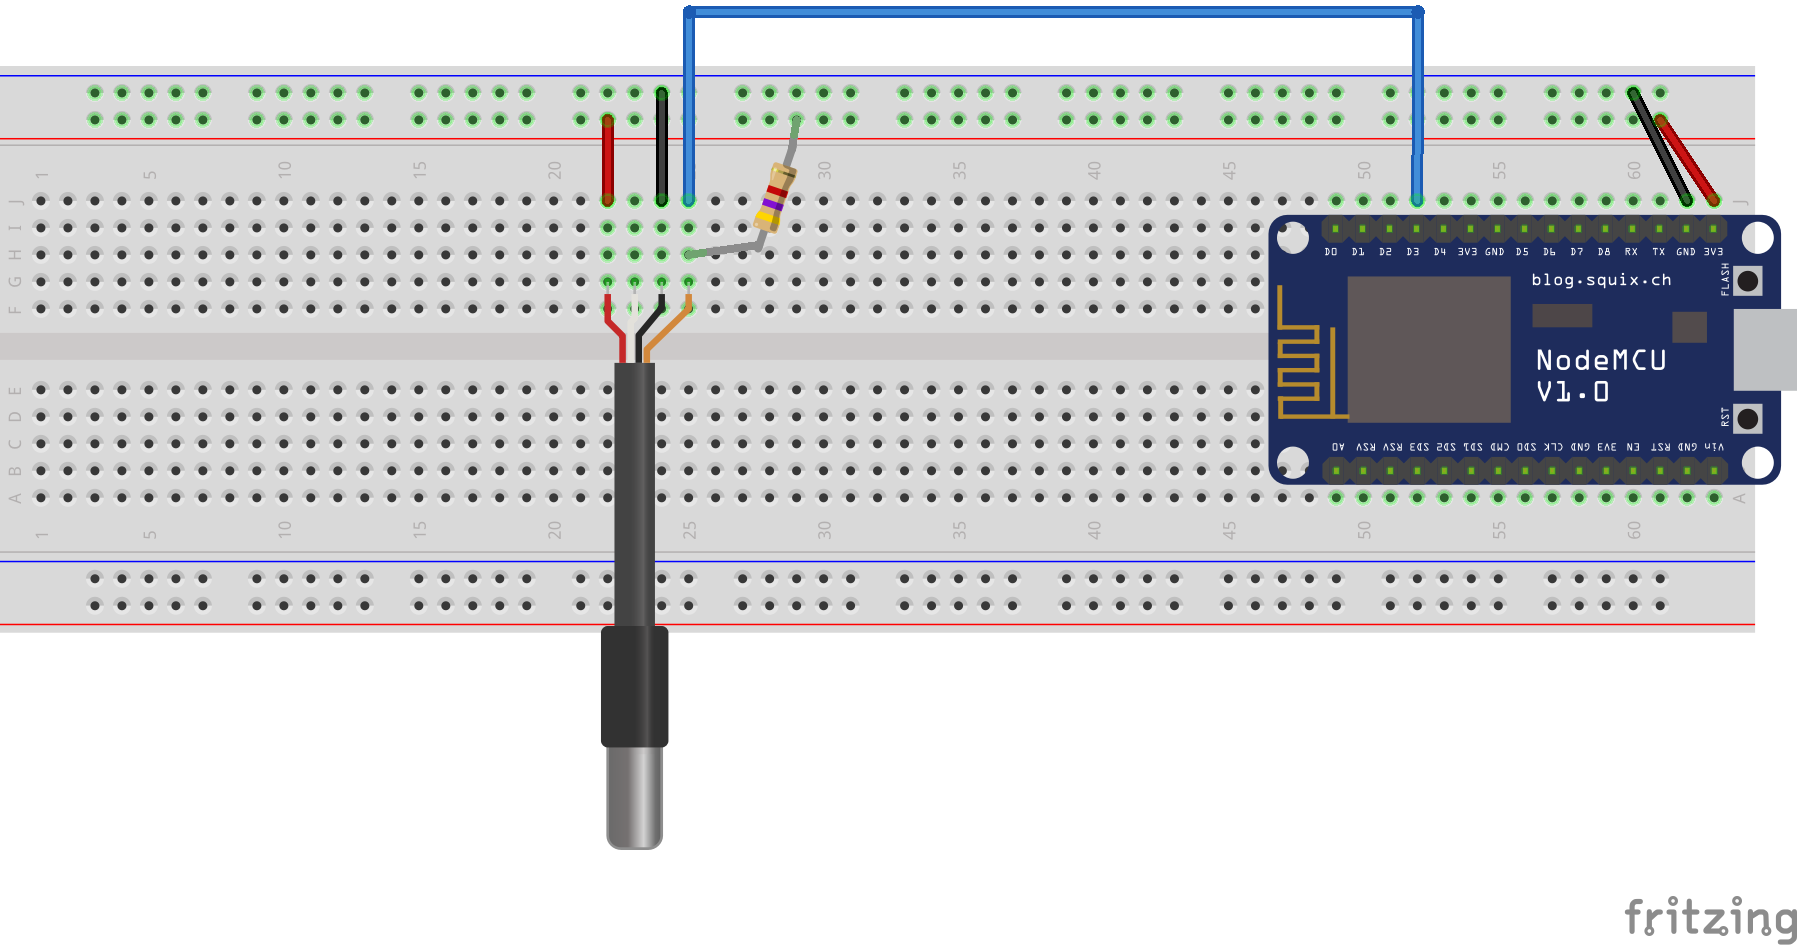
\includegraphics[width=\textwidth]{img/ds18b20_schema.png}
	\caption{DS18B20 wiring diagram}
	\label{fig:ds18b20_schema}
\end{figure}

\subsection{TSL2591}

The TSL2591 \citep{TSL2591:Datasheet} is a light intensity sensor that converts the light intensity into a digital output transmitted by the I2C bus. The module's output is the value of light intensity in the lux unit with an accuracy of 4 decimal places, and the measuring range is from 188 $\mu$Lux to 88,000 Lux. The value of the sensor is measured to three decimal places, although it is not necessary to have such high accuracy. The module guarantees measurement accuracy in temperature conditions from -30 $^{\circ}$C to +80 $^{\circ}$C. The sensor is supplied with power from a 3.3 V output on the microchip and grounded to the microchip. The SDA and SCL outputs are wired to the D1 and D2 pins of the microchip to provide I2C communication. The wiring diagram of the TSL2591 sensor is shown in \cref{fig:tsl2591_schema}

\begin{figure}[H]
	\centering
	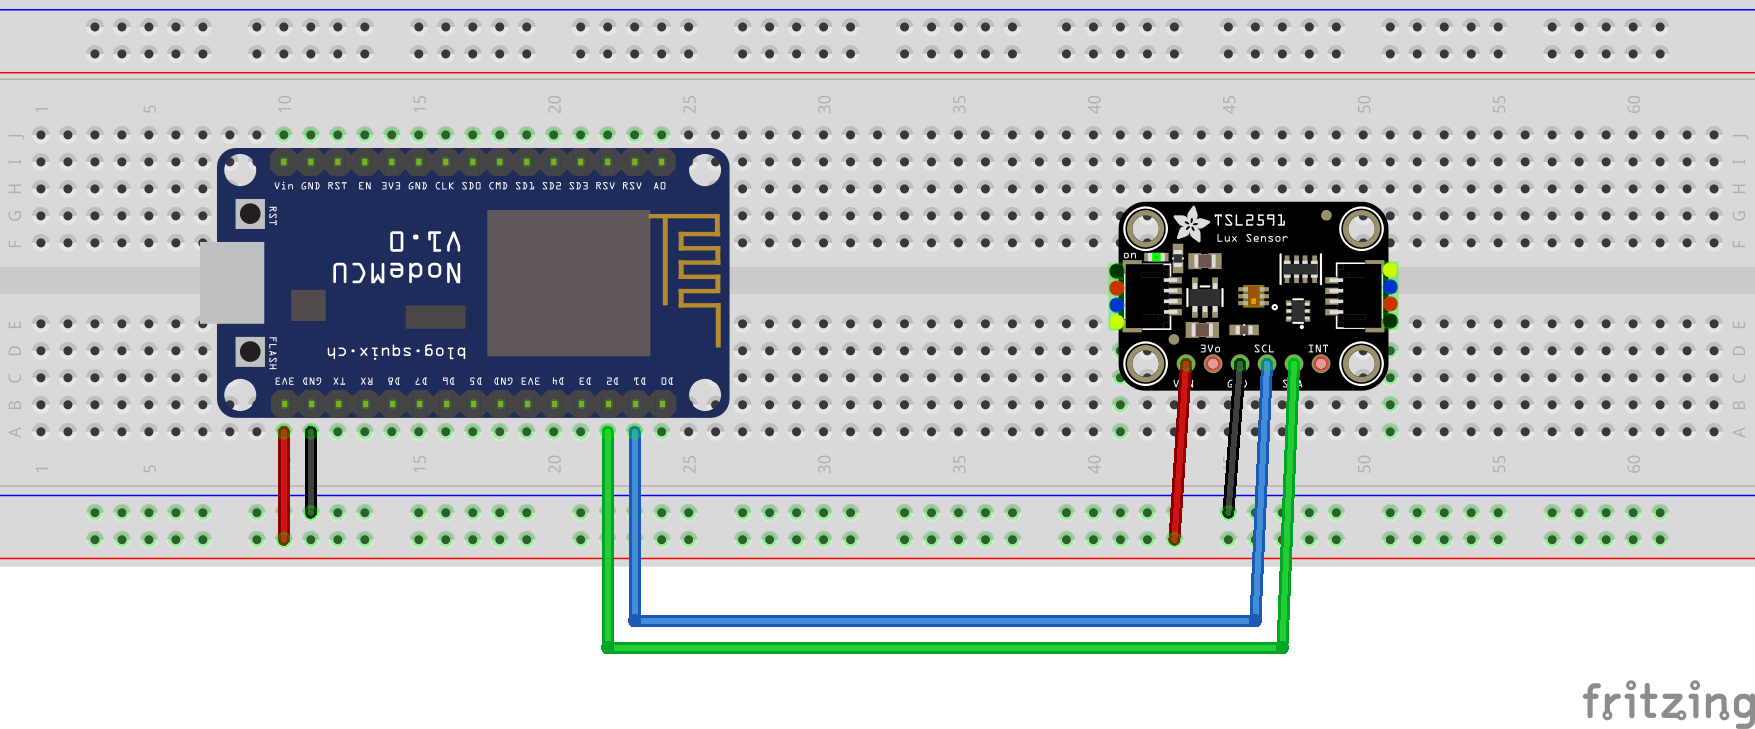
\includegraphics[width=\textwidth]{img/tsl2591_schema.png}
	\caption{TSL2591 wiring diagram}
	\label{fig:tsl2591_schema}
\end{figure}

\section{Time}

This module provides commands for manipulation with the time, such as asking for time, date, set timer. The module does not communicate with other devices. The module's functions exploit system information and information available on the Internet. To reach this information from the web is used technique call web scraping that can run the web site and suck desired pieces of information from this site. 

% A simple example of this technic is shown in \cref{lst:web_scraping_python}

% \begin{lstlisting}[language=python,firstnumber=1,caption={Simple example how to do web scraping in Python},captionpos=b, label={lst:web_scraping_python}]
%     from selenium import webdriver
%     from selenium.webdriver.chrome.options import Options

%     self.driver = webdriver.Chrome(executable_path='/usr/bin/chromedriver')
%     self.driver.get('www.seznam.cz')
% \end{lstlisting}

\subsection{Voice commands}
The module responds to the following questions:
\begin{itemize}
    \item Send command to ask the server for the current time\\
    \textbf{Voice commands}
    \begin{itemize}
        \item Kolik je hodin?
        \item Čas
    \end{itemize}
    \textbf{Reply}
    \begin{itemize}
        \item Právě je pět hodin dvacet minut a pět sekund.
    \end{itemize}
    \item Send command to ask the server for the current day of year\\
    \textbf{Voice commands}
    \begin{itemize}
        \item Kolikátého dnes je?
        \item Datum
    \end{itemize}
    \textbf{Reply}
    \begin{itemize}
        \item Dnes je 4. 5. 2021
    \end{itemize}
    \item Send a command to the server to start timer on 3 minute\\
    \textbf{Voice commands}
    \begin{itemize}
        \item Zapni časovač
    \end{itemize}
    \textbf{Reply}
    \begin{itemize}
        \item Časovač je nastaven na 3 minuty
    \end{itemize}
    \item Send a command to the server to stop timer\\
    \textbf{Voice commands}
    \begin{itemize}
        \item Vypni časovač
        \item Zastav časovač
    \end{itemize}
    \textbf{Reply}
    \begin{itemize}
        \item Časovač je vypnut
    \end{itemize}
    \item Ask the server for today's day of the week\\
    \textbf{Voice commands}
    \begin{itemize}
        \item Co je za den v týdnu?
        \item Co je za den?
    \end{itemize}
    \textbf{Reply}
    \begin{itemize}
        \item Dnes je pondělí.
    \end{itemize}
    \item Ask the server for today's sunrise time\\
    \textbf{Voice commands}
    \begin{itemize}
        \item Kdy vychází slunce?
        \item Východ slunce
    \end{itemize}
    \textbf{Reply}
    \begin{itemize}
        \item Nebylo možno získat data ze serveru meteogram.cz
        \item Slunce vychází v šest hodin a třicet minut.
    \end{itemize}
    \item Ask the server for today's sunset time\\
    \textbf{Voice commands}
    \begin{itemize}
        \item Kdy zapadá slunce?
        \item Západ slunce
    \end{itemize}
    \textbf{Reply}
    \begin{itemize}
        \item Nebylo možno získat data ze serveru meteogram.cz
        \item Slunce zapadá v osmnáct hodin a třicet minut.
    \end{itemize}
    \item Ask the server for today's nameday\\
    \textbf{Voice commands}
    \begin{itemize}
        \item Kdo má dnes svátek?
        \item Svátek
    \end{itemize}
    \textbf{Reply}
    \begin{itemize}
        \item Nebylo možno získat data ze serveru svatky.centrum.cz
        \item Podle serveru svatky.centrum.cz Renata.
    \end{itemize}
\end{itemize}

\section{System}

The system module provides the user commands to test the functionality and adjust some settings of the engine. The module communicates primarily with the engine, but it is possible to establish this communication with other devices. Like other technology, the module uses the MongoDB library from python to test the engine's database.

\begin{itemize}
    \item Reloads all the modules again. A fresh refresh.\\
    \textbf{Voice commands}
    \begin{itemize}
        \item Načti moduly
        \item Aktualizuj moduly
        \item Přenačti moduly
    \end{itemize}
    \textbf{Reply}
    \begin{itemize}
        \item Moduly byly znovu načteny.
    \end{itemize}
    \item Makes a testing write and read with the database.\\
    \textbf{Voice commands}
    \begin{itemize}
        \item Otestuj databáze
        \item Test databáze
        \item Otestuj databázi
    \end{itemize}
    \textbf{Reply}
    \begin{itemize}
        \item Modul System: Databáze otestována. Vyhledáno dat jeden.
        \item Modul System: Chyba při testování databáze
    \end{itemize}
    \item Makes a testing MQTT publish to voicehome/system/test, which this module is also subscribing\\
    \textbf{Voice commands}
    \begin{itemize}
        \item Otestuj MQTT
        \item Test MQTT
        \item Vyzkoušej MQTT
    \end{itemize}
    \textbf{Reply}
    \begin{itemize}
        \item Na mqtt nebylo možné odesla zprávu
        \item Zpráva na mqtt odeslána
    \end{itemize}
    \item Sends a testing websocket message with passport system/test.\\
    \textbf{Voice commands}
    \begin{itemize}
        \item Otestuj WebSocket
        \item Test WebSocket
        \item Vyzkoušej WebSockety
    \end{itemize}
    \textbf{Reply}
    \begin{itemize}
        \item Na websoket nebylo možné odesla zprávu
        \item Zpráva na websoket odeslána
    \end{itemize}
\end{itemize}

\section{Weather}

The weather module provides the user commands to answer questions about the weather. The module's functions exploit the information available on the Internet. By preprocessing the information from the Internet and replating characters like "°C" to "stupnů" or "-" to "mínus", we can then send fully synthesizable text to SpeechCloud and answer the question to the user. To reach this information from the web is used technique call web scraping that can run the web site and suck desired pieces of information from this site. Preprocessing the information uses the technique regex and essential functions such as finding text and selecting text — a simple example of how regex is used shown in \cref{lst:regex_python}.

% \lstinputlisting[language=python,firstnumber=1,caption={Simple example how to use regex in Python},captionpos=b, label={lst:regex_python}]{code/regex_example.py}


\begin{itemize}
    \item Getting forecast for today from www.chmi.cz.\\
    \textbf{Voice commands}
    \begin{itemize}
        \item Dnešní předpověď
        \item Jak dnes bude?
    \end{itemize}
    \textbf{Reply}
    \begin{itemize}
        \item Nebylo možno získat data ze serveru chmi.cz
        \item Server chmi.cz předpovídá pro dnešek. Polojasno až oblačno, místy přeháňky...
    \end{itemize}
    \item Getting forecast for tomorrow from www.chmi.cz.\\
    \textbf{Voice commands}
    \begin{itemize}
        \item Předpověď zítra
        \item Jak zítra bude?
    \end{itemize}
    \textbf{Reply}
    \begin{itemize}
        \item Nebylo možno získat data ze serveru chmi.cz
        \item Server chmi.cz předpovídá pro zítřek. Polojasno až oblačno, místy přeháňky...
    \end{itemize}
    \item Getting forecast for monday from www.chmi.cz if it is up to four days and not today.\\
    \textbf{Voice commands}
    \begin{itemize}
        \item Předpověď na pondělí
        \item Jak bude pondělí?
    \end{itemize}
    \textbf{Reply}
    \begin{itemize}
        \item Nebylo možno získat data ze serveru chmi.cz
        \item Server chmi.cz předpovídá na pondělí. Polojasno až oblačno, místy přeháňky...
    \end{itemize}
    \item Getting forecast for tuesday from www.chmi.cz if it is up to four days and not today.\\
    \textbf{Voice commands}
    \begin{itemize}
        \item Předpověď na úterý
        \item Jak bude úterý?
    \end{itemize}
    \textbf{Reply}
    \begin{itemize}
        \item Nebylo možno získat data ze serveru chmi.cz
        \item Server chmi.cz předpovídá na úterý. Polojasno až oblačno, místy přeháňky...
    \end{itemize}
    \item Getting forecast for wednesday from www.chmi.cz if it is up to four days and not today.\\
    \textbf{Voice commands}
    \begin{itemize}
        \item Předpověď na středu
        \item Jak bude středu?
    \end{itemize}
    \textbf{Reply}
    \begin{itemize}
        \item Nebylo možno získat data ze serveru chmi.cz
        \item Server chmi.cz předpovídá na středu. Polojasno až oblačno, místy přeháňky...
    \end{itemize}
    \item Getting forecast for thursday from www.chmi.cz if it is up to four days and not today.\\
    \textbf{Voice commands}
    \begin{itemize}
        \item Předpověď na čtvrtek
        \item Jak bude čtvrtek?
    \end{itemize}
    \textbf{Reply}
    \begin{itemize}
        \item Nebylo možno získat data ze serveru chmi.cz
        \item Server chmi.cz předpovídá na čtvrtek. Polojasno až oblačno, místy přeháňky...
    \end{itemize}
    \item Getting forecast for friday from www.chmi.cz if it is up to four days and not today.\\
    \textbf{Voice commands}
    \begin{itemize}
        \item Předpověď na pátek
        \item Jak bude pátek?
    \end{itemize}
    \textbf{Reply}
    \begin{itemize}
        \item Nebylo možno získat data ze serveru chmi.cz
        \item Server chmi.cz předpovídá na pátek. Polojasno až oblačno, místy přeháňky...
    \end{itemize}
    \item Getting forecast for saturday from www.chmi.cz if it is up to four days and not today.\\
    \textbf{Voice commands}
    \begin{itemize}
        \item Předpověď na sobotu
        \item Jak bude sobotu?
    \end{itemize}
    \textbf{Reply}
    \begin{itemize}
        \item Nebylo možno získat data ze serveru chmi.cz
        \item Server chmi.cz předpovídá na sobotu. Polojasno až oblačno, místy přeháňky...
    \end{itemize}
    \item Getting forecast for sunday from www.chmi.cz if it is up to four days and not today.\\
    \textbf{Voice commands}
    \begin{itemize}
        \item Předpověď na neděli
        \item Jak bude neděli?
    \end{itemize}
    \textbf{Reply}
    \begin{itemize}
        \item Nebylo možno získat data ze serveru chmi.cz
        \item Server chmi.cz předpovídá na neděli. Polojasno až oblačno, místy přeháňky...
    \end{itemize}
\end{itemize}
